\documentclass[onecolumn,draftclsnofoot, 10pt, compsoc]{IEEEtran}

\usepackage{graphicx}
\usepackage[section]{placeins}
\usepackage{caption}

\usepackage{amssymb}                                         
\usepackage{amsmath}                                         
\usepackage{amsthm}                                

\usepackage{alltt}                                           
\usepackage{float}
\usepackage{color}
\usepackage{url}

\usepackage{balance}
\usepackage[TABBOTCAP, tight]{subfigure}
\usepackage{enumitem}
\usepackage{pstricks, pst-node}
\usepackage{url}
\usepackage{setspace}

\usepackage{etoolbox}
\AtBeginEnvironment{quote}{\singlespacing\vspace{-\topsep}\small}

%\input{pygments.tex}

\usepackage{geometry}
\geometry{left=0.75in,right=0.75in,top=0.75in,bottom=0.75in}
\parindent = 0.0 in
\parskip = 0.1 in


\def \ParSpace{\vspace{.75em}}
\def \Jeremy{			Jeremy Fischer}
\def \Class{		Parallel Programming}
\def \Assn{		Project 4: Functional Decomposition ("Grainville")}
\def \School{	Oregon State University}
\def \Professor{		Matthew Meyn}

\newcommand{\cred}[1]{{\color{red}#1}}
\newcommand{\cblue}[1]{{\color{blue}#1}}

\newcommand{\NameSigPair}[1]{
		\par
		\makebox[2.75in][r]{#1} \hfil 	\makebox[3.25in]{\makebox[2.25in]{\hrulefill} \hfill			
		\makebox[.75in]{\hrulefill}}
		\par\vspace{-12pt} \textit{
			\tiny\noindent
			\makebox[2.75in]{} \hfil		
			\makebox[3.25in]{
				\makebox[2.25in][r]{Signature} \hfill	\makebox[.75in][r]{Date}
			}
		}
}










%%%%%%%%%%%%%%%%%%%%%%%%%%%%%%%%%%%%%%%
\begin{document}
\begin{titlepage}
    \pagenumbering{gobble}
    \begin{singlespace}
    	
\includegraphics[height=4cm]{coe.eps}
        \hfill  
        \par\vspace{.2in}
        \centering
        \scshape{
            \vspace{.5in}
            \textbf{\Large\Assn}\par
            \textbf{\large\Class}\par
            \large{
            	\today \\Spring Term
        	}
            \vfill
            {\large Prepared for}\par
            \huge \School\par
            \vspace{5pt}
            {\Large{\Professor}\par}
            {\large Prepared by }\par

            \vspace{5pt}
            {\Large
                {\Jeremy}\par
            }
            \vspace{20pt}
        }

    \end{singlespace}
\end{titlepage}
\newpage
\pagenumbering{arabic}

% 7. uncomment this (if applicable). Consider adding a page break.
%\listoffigures
%\listoftables
\clearpage







	\section{Custom Agent}
		The agent that I created to disturb the grain growth was "Locust Outburst."
		Essentially, if the current month is between May and September then a random percentage between 0 and 1 is generated.
		If the percentage is greater or equal to 75\%, then the grain is destroyed by a random number between the current height of the grain and a half of an inch.
		To do this I added an additional \textit{omp barrier} that handles the \textit{Is there a locust outburst this harvest?} question.
		Then, the function that calculates how much grain grows calls the function that incorporates the harm done by locust if there was an outburst.
	
	
	
	
	
	\section{Results Table}
	Since the total table is 72 columns long  due to the 72 month long simulation, I only posted the first 12 months.
	This along with the graph below in the \textit{Results Graph} section should shine light on the type of values that I was getting in the simulation.
	\textbf{Note} that the \textit{Precipitation} and \textit{Grain Height} values are in centimeters, \textit{Temperature} is in Celsius, and \textit{Locust} is 1 when there was a locust outburst and 0 if not.
	
		\begin{center}
			\begin{tabular}{|c|c|c|c|c|c|}
				\hline
				
				\textbf{Month} & \textbf{Precipitation} & \textbf{Temperature} & \textbf{Grain Height} & \textbf{Number of Deer} & \textbf{Locust} \\ \hline
			0 & 14.241253 & -3.59275 &1.270001&1&0 \\ \hline
			1 & 25.149177	& 0.844801&2.066129&0	&0\\ \hline
			2 &34.970879	&2.321667&15.41841&1&0\\ \hline
			3 & 32.656541	&12.701412&29.383819	&2&0\\ \hline
			4 & 30.411932	&12.644914&28.90038&3&0\\ \hline
			5 & 18.968795	&21.747284&27.302265&4&1\\ \hline
			6 & 7.384537	&23.350868&0&5&1\\ \hline
			7 & 8.611112	&19.393408&0&4&0\\ \hline
			8 & 0	&10.264339&0	&3&0\\ \hline
			9 & 0&7.586678&0&2&0\\ \hline
			10 & 0 	&7.692875&2.888701&1&0\\ \hline
			11 & 14.876699 &3.073016&6.929334&2&0\\ \hline
			\dots & \dots & \dots & \dots & \dots & \dots  \\ \hline
			\end{tabular}
		\end{center}
	
	
	
	
	
	
	\section{Results Graph}

	\begin{figure}[H]
		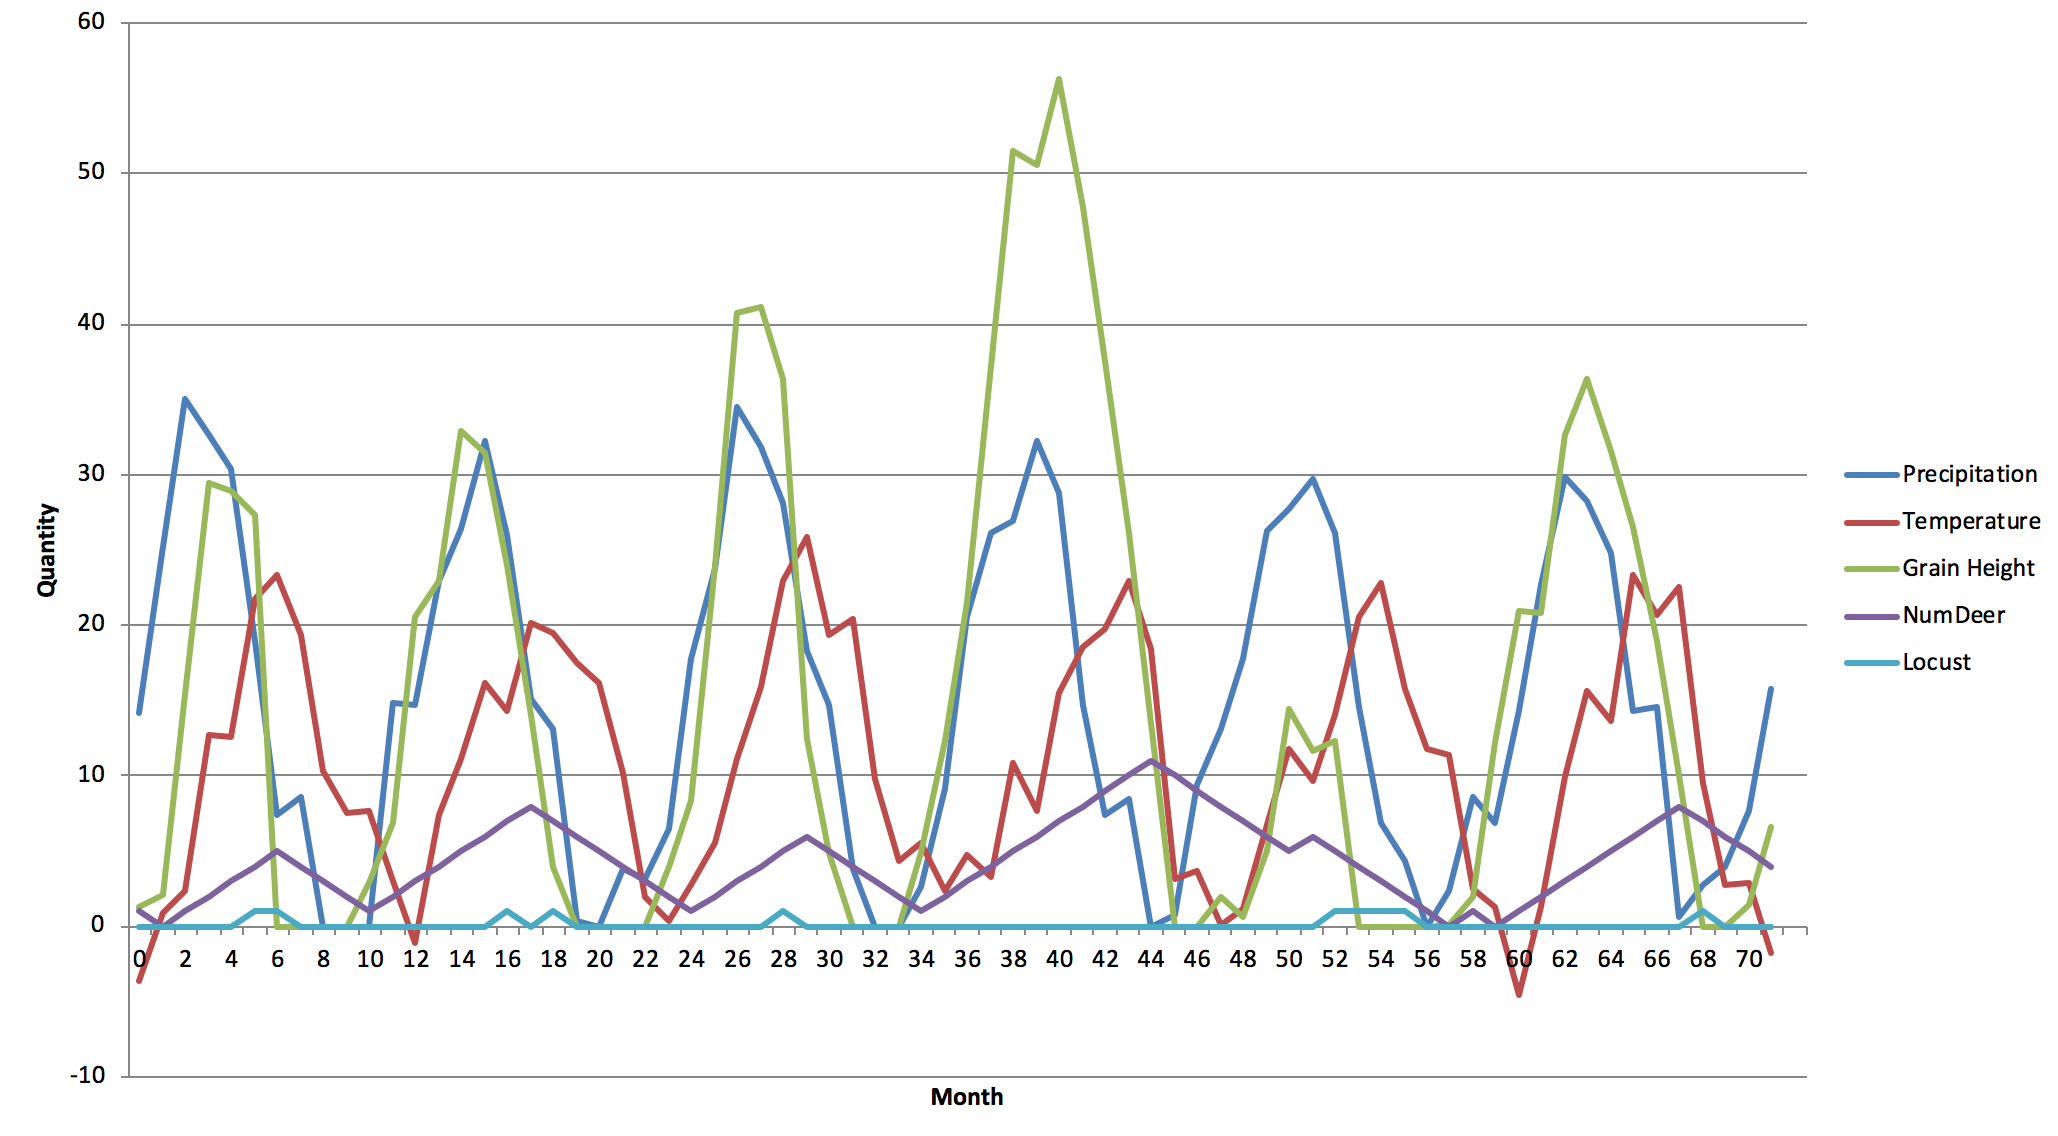
\includegraphics[width=18cm]{Graph}
		\centering
		\caption{Graph for Grainsville. \textbf{Note} that the \textit{Precipitation} and \textit{Grain Height} values are in centimeters, \textit{Temperature} is in Celsius, and \textit{Locust} is 1 when there was a locust outburst and 0 if not.}
	\end{figure}

	
\section{Why do you think it is behaving this way?}
	The fact that all of the curves (besides the locust curve) reflects a cyclical, sinusoidal, curve shape shows that all four of the threads were on the same page.
	Meaning, they stopped at the the \textit{omp barrier}'s and waited until all threads made it to the barrier before continuing.
	If this were not the case then there would be random spikes and dips because the threads would be using different values for the global variables.
	One can also see that the number of deer is dependent on the grain height which is dependent upon the temperature and precipitation.
	This is shown by the way the curves follow each other.
	


\end{document}